\documentclass[12pt,halfline,a4paper]{ouparticle}

\usepackage{lmodern}
\usepackage[T1]{fontenc}
\usepackage{textcomp}

\usepackage{graphicx}
\graphicspath{ {../grafici/} }

\begin{document}

\title{Report\break {Sistemi di Calcolo Parallelo e Applicazione}}

\author{%
\name{Valerio Cristofori}
%\address{Institute or Organization, Department, City, State,\\
%Zip Code, Country}
%\email{e-mail address}
%\and
%\name{Second Author}
%\address{Institute or Organization, Department, City, State,\\
%Zip Code, Country}
%\email{e-mail address}
}

\abstract{This sample is a guideline for preparing technical papers using \LaTeX\
for manuscript submission. It contains the documentation for your \LaTeX\
Class file, which implements the layout for your manuscript for all Journals of OUP.
This sample article uses a class file named \texttt{ouparticle.cls} that all authors
need to use for their manuscript preparation. It is similar in use to the \texttt{article}
class file of \LaTeX, but has some extra fields in the preamble and some extended commands for
other parts of the article.}

\date{24 Febbraio 2022}

\maketitle

\section{Introduzione}
\label{sec1}

It is assumed that the author is familiar with either plain
\TeX, \AmS-\TeX{} or a standard \LaTeX\ setup and, hence,
only the essential points are described in this document.
Nevertheless, we hope that this document is generally sufficient
for describing the requirements for preparation of
manuscripts. For more details, please see the \textit{\LaTeX{} User's Guide} or
\textit{The not so short introduction to \LaTeXe}.


\section{Progettazione}
\label{sec2}

Provided with \verb+ouparticle.cls+ are the files
\verb+sample.tex+ (this document explains the various
features of \verb+ouparticle.cls+) and \verb+sample.pdf+
(how the output using \verb+sample.tex+ should be). Your
paper can be compiled with standard \LaTeX,
preferably with the current \LaTeXe\ version. It will probably work
with older versions of \LaTeXe; however, this has not been
tested. The file \verb+ouparticle.cls+ needs to be copied
into a directory where \TeX\ looks for input files. The other files
need to be kept as a reference while preparing
your manuscript. Please use the predefined commands from \verb+sample.tex+ for title,
authors, abstract, body, etc.


\section{Implementazione}
\label{sec3}

\subsection{Calcolo Seriale}
\label{sec3.1}


\begin{center}
\begin{tabular}{|| c | c | c ||} 
\hline
Matrice & Speedup CPU & d \\ [1ex]
\hline
adder\_dcop\_32 & 0.21 & 0.01 \\
\hline
af\_1\_k101 & 9.68 & 8.80 \\
\hline
af23560 & 2.92 & 2.77 \\
\hline
amazon0302 & 5.81 & 5.83 \\
\hline
bcsstk17 & 1.71 & 1.07 \\
\hline
cage4 & 0.00 & 0.00 \\
\hline
cant & 4.74 & 5.92 \\
\hline
cavity10 & 0.53 & 0.47 \\
\hline
cop20k\_A & 7.09 & 2.66 \\
\hline
Cube\_Coup\_dt0 & 10.14 & 7.99 \\
\hline
dc1 & 2.31 &  \\
\hline
FEM\_3D\_thermal1 & 2.28 & 2.39 \\
\hline
lung2 & 3.26 & 2.43 \\
\hline
mac\_econ\_fwd500 & 3.69 & 1.29 \\
\hline
mcfe & 0.23 & 0.18 \\
\hline
mhd4800a & 0.73 & 0.65 \\
\hline
mhda416 & 0.12 & 0.04 \\
\hline
ML\_Laplace & 9.96 & 9.01 \\
\hline
nlpkkt80 & 9.74 & 8.75 \\
\hline
olafu & 3.39 & 3.20 \\
\hline
olm1000 & 0.05 & 0.06 \\
\hline
PR02R & 8.47 & 4.58 \\
\hline
raefsky2 & 1.48 & 1.23 \\
\hline
rdist2 & 0.48 & 0.23 \\
\hline
roadNet-PA & 5.93 & 3.20 \\
\hline
thermal1 & 2.31 & 3.44 \\
\hline
thermal2 & 3.93 & 5.57 \\
\hline
thermomech\_TK & 4.53 & 4.24 \\
\hline
webbase-1M & 6.09 &  \\
\hline
west2021 & 0.10 & 0.08 \\
\hline
\end{tabular}
\end{center}



\begin{center}
\begin{tabular}{|| c | c | c ||} 
\hline
Matrice & Speedup GPU \\ [1ex]
\hline
adder\_dcop\_32 & 1.78 & 0.78 \\
\hline
af\_1\_k101 & 66.32 & 110.73 \\
\hline
af23560 & 35.67 & 72.48 \\
\hline
amazon0302 & 21.79 & 72.35 \\
\hline
bcsstk17 & 26.97 & 46.71 \\
\hline
cage4 & 0.00 & 0.00 \\
\hline
cant & 75.58 & 81.33 \\
\hline
cavity10 & 6.81 & 17.19 \\
\hline
cop20k\_A & 50.65 & 69.95 \\
\hline
Cube\_Coup\_dt0 & 110.93 & 119.84 \\
\hline
dc1 & 8.32 &  \\
\hline
FEM\_3D\_thermal1 & 28.77 & 61.26 \\
\hline
lung2 & 9.68 & 24.02 \\
\hline
mac\_econ\_fwd500 & 16.89 & 32.47 \\
\hline
mcfe & 2.41 & 4.21 \\
\hline
mhd4800a & 10.38 & 23.35 \\
\hline
mhda416 & 1.25 & 2.27 \\
\hline
ML\_Laplace & 113.11 & 115.12 \\
\hline
nlpkkt80 & 69.91 & 109.88 \\
\hline
olafu & 53.04 & 79.07 \\
\hline
olm1000 & 0.52 & 1.28 \\
\hline
PR02R & 81.70 & 65.85 \\
\hline
raefsky2 & 18.29 & 39.91 \\
\hline
rdist2 & 4.83 & 11.35 \\
\hline
roadNet-PA & 14.93 & 106.62 \\
\hline
thermal1 & 16.81 & 39.09 \\
\hline
thermal2 & 30.21 & 111.85 \\
\hline
thermomech\_TK & 21.35 & 48.29 \\
\hline
webbase-1M & 13.11 &  \\
\hline
west2021 & 0.70 & 2.00 \\
\hline
\end{tabular}
\end{center}


\begin{center}
\begin{tabular}{|| c | c | c ||} 
\hline
Matrice & GFlops CPU \\ [1ex]
\hline
adder\_dcop\_32 & 0.04 & 0.00 \\
\hline
af\_1\_k101 & 4.67 & 4.24 \\
\hline
af23560 & 1.10 & 1.10 \\
\hline
amazon0302 & 1.02 & 1.30 \\
\hline
bcsstk17 & 0.85 & 0.49 \\
\hline
cage4 & 0.00 & 0.00 \\
\hline
cant & 2.31 & 2.44 \\
\hline
cavity10 & 0.21 & 0.17 \\
\hline
cop20k\_A & 2.26 & 0.86 \\
\hline
Cube\_Coup\_dt0 & 5.04 & 3.99 \\
\hline
dc1 & 0.86 &  \\
\hline
FEM\_3D\_thermal1 & 0.92 & 0.94 \\
\hline
lung2 & 1.07 & 0.49 \\
\hline
mac\_econ\_fwd500 & 1.48 & 0.46 \\
\hline
mcfe & 0.08 & 0.04 \\
\hline
mhd4800a & 0.25 & 0.21 \\
\hline
mhda416 & 0.03 & 0.03 \\
\hline
ML\_Laplace & 4.83 & 4.36 \\
\hline
nlpkkt80 & 4.67 & 4.24 \\
\hline
olafu & 1.65 & 1.42 \\
\hline
olm1000 & 0.02 & 0.02 \\
\hline
PR02R & 4.14 & 2.25 \\
\hline
raefsky2 & 0.46 & 0.39 \\
\hline
rdist2 & 0.15 & 0.07 \\
\hline
roadNet-PA & 1.38 & 0.75 \\
\hline
thermal1 & 1.17 & 1.02 \\
\hline
thermal2 & 0.93 & 1.60 \\
\hline
thermomech\_TK & 1.13 & 0.99 \\
\hline
webbase-1M & 1.66 &  \\
\hline
west2021 & 0.03 & 0.03 \\
\hline
\end{tabular}
\end{center}


\begin{center}
\begin{tabular}{|| c | c | c ||} 
\hline
Matrice & GFlops GPU \\ [1ex]
\hline
adder\_dcop\_32 & 0.44 & 0.19 \\
\hline
af\_1\_k101 & 31.85 & 53.18 \\
\hline
af23560 & 15.37 & 31.24 \\
\hline
amazon0302 & 4.86 & 16.14 \\
\hline
bcsstk17 & 12.07 & 20.91 \\
\hline
cage4 & 0.01 & 0.01 \\
\hline
cant & 35.46 & 38.17 \\
\hline
cavity10 & 2.88 & 7.27 \\
\hline
cop20k\_A & 18.10 & 24.99 \\
\hline
Cube\_Coup\_dt0 & 53.89 & 58.22 \\
\hline
dc1 & 3.30 &  \\
\hline
FEM\_3D\_thermal1 & 13.05 & 27.79 \\
\hline
lung2 & 3.75 & 9.29 \\
\hline
mac\_econ\_fwd500 & 6.40 & 12.30 \\
\hline
mcfe & 1.00 & 1.74 \\
\hline
mhd4800a & 4.54 & 10.23 \\
\hline
mhda416 & 0.43 & 0.78 \\
\hline
ML\_Laplace & 53.51 & 54.45 \\
\hline
nlpkkt80 & 33.36 & 52.43 \\
\hline
olafu & 24.76 & 36.91 \\
\hline
olm1000 & 0.18 & 0.44 \\
\hline
PR02R & 38.61 & 31.12 \\
\hline
raefsky2 & 8.17 & 17.83 \\
\hline
rdist2 & 2.11 & 4.95 \\
\hline
roadNet-PA & 3.60 & 25.70 \\
\hline
thermal1 & 5.55 & 12.91 \\
\hline
thermal2 & 8.91 & 33.00 \\
\hline
thermomech\_TK & 5.67 & 12.82 \\
\hline
webbase-1M & 3.89 &  \\
\hline
west2021 & 0.23 & 0.67 \\
\hline
\end{tabular}
\end{center}

\subsection{Calcolo con OpenMP}
\label{sec3.2}

Before you type anything that actually appears in the paper, you need to
include a \verb+\documentclass{ouparticle}+ command at the very beginning,
and then the two commands that have to be part of any \LaTeX\ document,
\verb+\begin{document}+ at the start and \verb+\end{document}+ at the
end of your paper.


\subsection{Calcolo con CUDA}
\label{sec3.3}

The main structure of your paper is as follows:


\section{Performance}
\label{sec4}

By default, all of the options within \verb+article.cls+ are available
with this class file. This class file provides the following additional options.


\subsection{Front matter}
\label{sec4.1}

The title of the manuscript is simply specified by using the \verb+\title{text}+ command in
the same manner as in this sample. Author's information consists of the name of the author
and the corresponding institutions with addresses, as given in this example. Include an
electronic mail address if available, inserting it into the \verb+\email{text}+ commands.
You may follow the same coding if there are more than one author; separate authors with
\verb+\and+. Please identify the corresponding author with his/her electronic
mail address by \verb+\thanks{text}+. An abstract for your paper is specified by using
\verb+\abstract{text}+. A \verb+\keywords{text}+ macro may also be used to indicate keywords for the
article. Use \verb+\maketitle+ after the abstract and keywords to make the header of your article.

\subsection{Sections and subsections}
\label{sec4.2}

To begin a new section, give the heading of that section in the \verb+\section{text}+ command.
A section number is supplied automatically. Use the starred form (\verb+\section*{text}+) of the
command to suppress the automatic numbering. If you want to be able to make reference to that section,
then you need to \texttt{label} it (see Section \ref{sec3.14}). You can have sections up to
five levels. The sectioning commands are \verb|\section|, \verb|\subsection|, \verb|\subsubsection|,
\verb|\paragraph| and \verb|\subparagraph|.

\section{Conclusioni}
\label{sec5}

The ends of words and sentences are marked by spaces. It does not matter how many
spaces you type. The end of a line counts as a space. One
or more blank lines denote the end of a paragraph.


\subsection{Appendix}
\label{sec6.1}

The \verb+\appendix+ command signals that all following sections are
appendices, and therefore the headings after \verb+\appendix+ will be set
as appendix headings. For a single appendix, use \verb+\appendix*+ followed by the \verb+\section{text}+
command to suppress the appendix letter in the section heading.




\section{References}
\label{sec6}

The reference entries can be \LaTeX\ typed bibliographies or generated through a BIB\TeX\ database.
BIB\TeX\ is an adjunct to \LaTeX\ that aids in the preparation of bibliographies. BIB\TeX\
allows authors to build up a database or collection of bibliography entries that may be used for many
manuscripts. They also save us the trouble of having to specify formatting. More details can be found
in the \textit{BIB\TeX\ Guide}. For \LaTeX\ reference entries use the
\verb+\begin{thebibliography}....\end{thebibliography}+ environment (see below) to make references in your paper.
We have provided the class file option to distinguish two styles of references. Those options are \verb+numbib+ and \verb+nonumbib+.
You can select one of these options with the \verb+\documentclass+ command. By default the class file will take the
\verb+numbib+ option. The following is an example of \LaTeX\ bibliography.

\begin{verbatim}
\begin{thebibliography}{0}
\bibitem{bib1}
Goossens, M., F. Mittelbach, and A. Samarin: {\em The {\LaTeX} Companion}.
Addison-Wesley, Reading, MA, USA, 1994.
\bibitem{bib2}
Knuth, D.E: {\em The {\TeX}book}. Addison-Wesley, Reading, MA, USA, 1984.
\bibitem{bib3}
Lamport, L.: {\em {\LaTeX} -- A Document Preparation System -- User's
Guide and Reference Manual}. Addison-Wesley, Reading, MA, USA, 1985.
\bibitem{bib4}
Smith, I.N., R.S. Johnes, and W.P. Hines: 1992, `Title of the Article',
\textit{Journal Title in Italics} \textbf{Vol. no. X}, pp. 00--00
\end{thebibliography}
\end{verbatim}


\begin{figure}[h]
\hspace*{-2.5cm} 
\centering
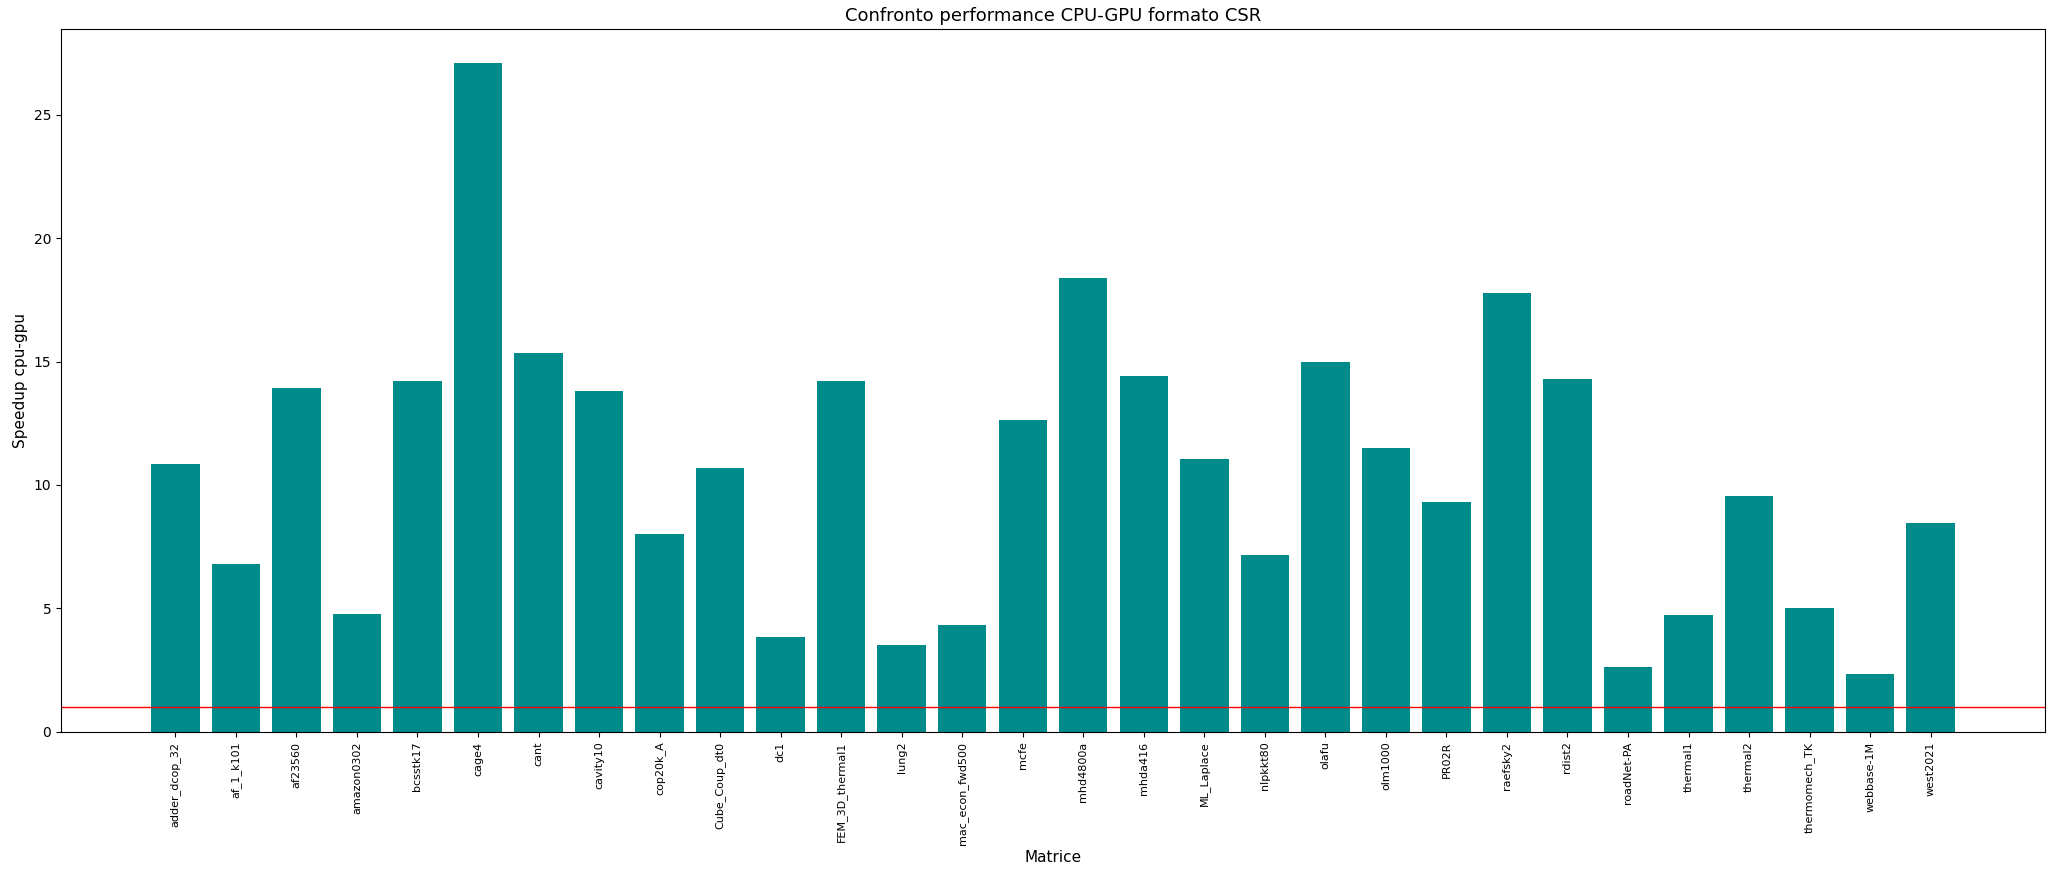
\includegraphics[width=20.5cm]{cpu-gpu-speedup-CSR}
\caption{here}
\end{figure}


\end{document}
